\section{Les lois a priori}
Lorsque l’on spécifie un modèle, on doit nécessairement fournir une distribution a priori pour les paramètres inconnus. Ces distributions jouent un rôle crucial dans l'inférence bayésienne grâce à l’équation de mise à jour
$$P(\theta\mid D) \propto P(\theta) \times P(D\mid \theta).$$ Dans l'approche bayésienne, toutes les quantités inconnues sont décrites de façon probabiliste, même avant que les données n'aient été observées.  \par Le choix d’une distribution a priori est \textbf{subjectif} (la décision d'utiliser une distribution spécifique est laissée à l'entière discrétion des analystes). Mais le choix de la distribution a priori \textbf{n'est ni plus ni moins subjectif que le choix de la vraisemblance, la sélection d'un échantillon, le cadre d’estimation, ou la statistique utilisée pour la réduction des données}.  \newl Le choix d'une distribution a priori peut cependant affecter considérablement les conclusions a posteriori, surtout lorsque la taille de l'échantillon est petite. \newl
Nous examinons maintenant quelques méthodes générales permettant de détermines les lois a priori.
\subsection{Lois a priori conjuguées}
La distribution a posteriori du vecteur $\theta$ pourrait tr\`es bien ne pas avoir de forme analytique -- c'est le principal défi des méthodes bayésiennes. \newl Plus précisément, il est souvent difficile, voir m\^eme math\'ematiquement impossible, de produire les distributions a posteriori marginales (c'est-\`a-dire, exprim\'ees \`a l'aide d'un unique param\`etre, et non des distributions conjointes) à partir d'une distribution a posteriori de grande dimension. \newpage\noindent Il y a cependant quelques exceptions permettant d'obtenir facilement des observation de la distribution a posteriori en utilisant une \textbf{distribution a priori conjuguée}. \par La conjugaison est une propriété commune d'une distre distribution a priori et d'un mod\`ele de vraisemblance; la distribution a posteriori correspondante prend la même forme que la distribution a priori, mais avec un ou des paramètre(s) différent(s). \newl Le tableau ci-dessous présente quelques vraisemblances communes et leur distribution a priori conjuguée (une liste d\'etaill\'ee se trouve dans ~\cite{BDA_N122}). 
\begin{center} 
\begin{tabular}{ccc} 
 \hline
  \textbf{Vraisemblance} & \textbf{A priori} & \textbf{Hyperparamètres} \\ \hline
 Bernouilli&Beta&$\alpha>0,\beta>0$
	\\  
 Binomiale&Beta&$\alpha>0,\beta>0$
	\\  
 Poisson&Gamma&$\alpha >0$, $\beta>0$
  \\  
 Normale -- $\mu$&Normale&$\mu\in\mathbb{R}$, $\sigma^{2}>0$
  \\  
 Normale -- $\sigma^{2}$&Gamma Inverse&$\alpha >0$, $\beta>0$
  \\  
 Exponentielle&Gamma&$\alpha >0$, $\beta>0$									
\\ \hline
\end{tabular}
\end{center}
Par exemple, si la probabilité de $s$ succès apr\`es $n$ tentatives (la vraisemblance) est donnée par $$P(s,n\mid q)=\frac{n!}{s!(n-s)!}q^s(1-q)^{n-s}, \quad q\in [0,1], $$ et la distribution a priori de $q$ suit une distribution $\text{Beta}(\alpha,\beta)$, $\alpha,\beta>0$, c'est-\`a-dire que $$P(q)=\frac{q^{\alpha-1}(1-q)^{\beta-1}}{B(\alpha,\beta)}, $$ pour $q\in [0,1]$, alors la distribution a posteriori de $q$ étant donné $s$ succès apr\`es $n$ tentatives suit une loi $\text{Beta}(\alpha+s,\beta+n-s)$: 
$$P(q\mid s,n)=\frac{P(s,n\mid q)\times P(q)}{P(s,n)}=\frac{q^{\alpha+s-1}(1-q)^{\beta+n-s-1}}{B(\alpha+s,\beta+n-s)}$$ pour $q\in [0,1]$. \newl 
Les distributions a priori conjuguées sont mathématiquement pratiques et assez flexibles, selon les hyperparamètres spécifiques qui sont utilis\'es, mais elles \textbf{reflètent des connaissances a priori très spécifiques}. On d\'econseille leur utilisation, à moins de posséder réellement ce savoir.

\subsection{Lois a priori non-informatives}
 Une distribution a priori non-informative est une distribution sur laquelle tr\`es peu d'éléments explicatifs sont fournis au sujet des paramètres inconnus.
Ces distributions sont très utiles dans la perspective du bayésianisme traditionnel qui cherche à atténuer la critique fréquentiste de la \textbf{subjectivité intentionnelle}. Ces a priori fournissent intentionnellement très peu d'informations spécifiques sur le(s) paramètre(s).  \newpage\noindent La distribution a priori non-informative classique est celle donn\'ee par la distribution uniforme sur une r\'egion finie. Par exemple, si les données suive une distribution de Bernoulli avec param\`etre $\theta$, la distribution uniforme sur $\theta$ est 
$$ P(\theta) = 1,\quad  0\leq\theta\leq 1.$$  Cette approche est sens\'ee lorsque $\theta$ a un support fini. Mais pour des données suivant une loi normale $N (\mu, 1)$, par exemple, la distribution a priori uniforme sur $-\infty<\mu<\infty$ est impropre car l'int\'egrale de $P(\mu)=a$ sur $\mathbb{R}$ diverge pour tout $a\neq 0$; cependant, un tel choix pourrait toujours être acceptable tant que la distribution a posteriori résultante est standardisée (c'est-à-dire que l'intégrale de la loi a posteriori converge sur son support). \par Comme il y a plusieurs cas où une distribution a priori impropre m\`ene a une distribution a posteriori aussi impropre, un soin est justifié.\newl   On justifie souvent la d\'ecision d’utiliser des lois a priori non-informatives par le principe qu'il faut  ``laisser les données parler d’elles-mêmes,'' de sorte que les inférences ne soient pas affectées par des pr\'ejug\'es qui ne sont pas soutenu par les données actuelles.

\subsection{Lois a priori informatives}
 Les a priori informatifs sont ceux qui insèrent \textbf{délibérément} les informations que les chercheurs ont sous la main. Cela semble être une approche raisonnable puisque les connaissances scientifiques antérieures devraient jouer un rôle dans l'inférence statistique . Cependant, il y a deux exigences importantes pour les chercheurs: \begin{enumerate}[noitemsep]
\item déclaration claire de spécifications a priori, et 
\item une analyse de sensibilité détaillée pour montrer l'effet de ces a priori par rapport aux types non informés.
\end{enumerate}
La transparence est nécessaire pour éviter l'écueil courant de le \textbf{(data fishing en anglais ou triturage de données)}; l'analyse de sensibilité peut donner une idée de la valeur informative exacte de la distribution a priori. Mais d'où viennent les a priori informatifs, en premier lieu? En général, ces a priori sont dérivés de:
\begin{itemize}[noitemsep]
	\item l'intuition du chercheur, des études effectuées par le passé, des articles publiées;
	\item interviewer des experts du domaine;
	\item la commodité avec la conjugaison, et 
	\item non paramétriques et d'autres sources dérivées de données.
\end{itemize}
L'information a priori qui provenant des études précédents n'ont pas besoins d'être en accord.  Une stratégie utile consiste à construire des spécifications a priori à partir \textbf{d'écoles de pensée concurrentes} afin de contraster les a priori qui en résultent et produire des déclarations éclairées sur la force relative de chacun d'eux. 

\begin{Exemple}\textbf{Influence de la distribution a priori.}  Nous avons noté précédemment qu'une vraisemblance de Bernoulli et un a priori bêta forment un ensemble de la distribution a priori conjugués. Pour cet exercice, nous utilisons la fonction R \texttt{BernBeta()} définie dans \cite{BDA_K} (notez que la fonction renvoie les valeurs bêta a posteriori à chaque appel, donc les valeurs renvoyées peuvent être réintroduites dans la distribution a priori lors du prochain appel de fonction).
\begin{enumerate}[label=(\alph*)]
	\item Commencez par une loi a priori qui exprime une certaine incertitude de l'équité d'une pièce de monnaies:$Beta(\theta\mid 4,4)$. Lancer la pièce de monnaie une fois et supposer qu'une face est obtenue.
Quelle est la loi a posteriori de l'incertitude dans l'équité de la pièce $\theta$? \newl 
	\textbf{Solution:} à l'invite de commande R, tapez: \newl \small \texttt{$> post = BernBeta(c(4,4) , c(1))$}\normalsize\newl Cette fonction utilise la relation de conjugaison de la Section 3.1 pour déterminer la loi a posteriori Beta pour l'incertitude de l'équité de la pièce de monnaies étant donné les paramètres de la Beta a priori et les données observées en supposant une vraisemblance de Bernouilli. (1 représente un F(ace) sur le lancement, 0 un P(ile) Cependant, nous savons sur des bases théoriques que la distribution a posteriori suit une loi  $\text{Beta}(\theta \mid  4+1,4+1-1)=\text{Beta}(\theta\mid  5,4)$.
	\begin{center}
	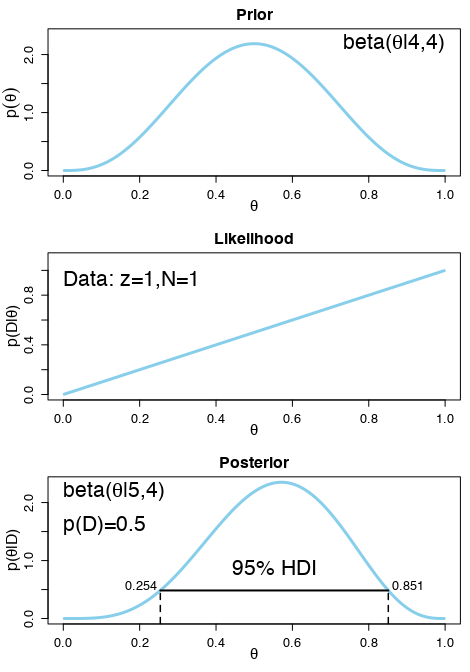
\includegraphics[width=\linewidth]{Images/example51.png}
	\end{center}
	La marque sur l'axe $y$ des ordonnées de la loi a posteriori fournit les paramètres a posteriori (ils sont également donnés en tapant \small \texttt{show(post)} \normalsize à l'invite de commande).
	
\item Utilisons les paramètres a posteriori du lancement précédent comme une a priori pour le lancement suivant. Supposons que nous retournions à nouveau et obtenions une $F$ . Quel est la nouvelle a posteriori sur l'incertitude de l'équité de la pièce de monnaies? \newl \textbf{Solution:} à l'invite de commande R, tapez
\newl \small \texttt{$> post = BernBeta(post , c(1))$}\normalsize\newl La loi a posteriori est  $\text{Beta}(\theta\mid 6,4)$, qui est indiquée ci- dessous. 
\begin{center}
	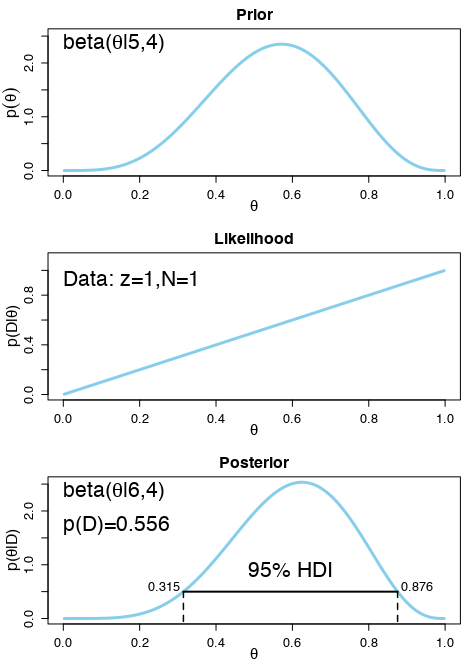
\includegraphics[width=\linewidth]{Images/example51b.png}
	\end{center} 
\item En utilisant le plus récent a posteriori comme a priori pour le lancement suivant, retournez une troisième fois et obtenez à nouveau une $F$. Quel est le nouveau a posteriori? \newl \textbf{Solution:} dans ce cas, nous savons que la distribution a posteriori pour l'équité de la pièce suit une loi  $\text{Beta}(\theta \mid 7,4)$ (nous ne fournirons ni le code ni la sortie, cette fois- ci!). Est-ce que 3 $F$ d'affilée vous font réfléchir? Est-ce qu'il a suffisamment de preuves pour suggérer que $\theta\neq 0.5$ (c'est-à-dire que la pièce n'est pas juste)? Et si vous retourniez 18 $F$ d'affilée à partir de ce moment?? 
\end{enumerate}
\label{ex4}
\end{Exemple} 
\noindent Lorsqu'on travaille sur un problème, il peut être facile de s'écarter et de se confondre avec la notation. Dans ces cas, il est utile de revenir à la définition de chacun des termes du théorème de Bayes. (c.à.d \@ $P(\theta\mid D)$, $P(D)$, $P(D\mid \theta)$, etc.).
\begin{Exemple} \textit{Un a priori inhabituel.} \label{Ex:unusualprior}
Supposons qu'une amie possède une pièce de monnaie dont nous savons qu'elle provient d'un magasin de magie; en conséquence, nous croyons que la pièce est fortement biaisée dans l'une ou l'autre des deux directions (il pourrait s'agir d'une pièce de monnaie truquée dont les deux faces seraient $F$, par exemple), mais nous ne savons pas laquelle elle favorise.  Nous exprimerons la croyance de cet a priori comme une loi Beta. Disons que notre amie retourne la pièce de monnaie cinq fois; ce qui donne 4 $F$ et 1 $P$. Quelle est la loi a posteriori de l'équité de la pièce de monnaie $\theta$? \newl 
\textbf{Solution}: à l'invite de commande R, tapez \newl \small \texttt{> post = BernBeta(c(1,1)/100,c(1,1,1,1,0))}\normalsize\newl 
donnant la distribution a posteriori ci-dessous.  
\begin{center}
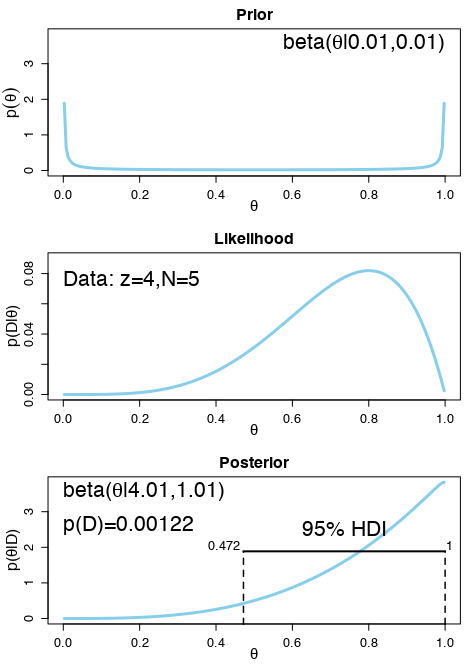
\includegraphics[width=\linewidth]{Images/example52.png}
\end{center}
Le code ci-dessus utilise un a priori donné par $\text{Beta}(\theta\mid 0.01,0.01)$. Cet a priori traduit notre conviction que la pièce est fortement biaisée (bien que nous ne sachions pas dans quelle direction se situe le biais avant de voir les données). Le choix de $0.01$ est arbitraire, dans un sens; 0.1 aurait également fonctionné, par exemple.  \par La loi a posteriori est donc $\text{Beta}(\theta\mid 4.01,1.01)$ qui, comme indiqué ci-dessus, a son mode essentiellement à $1.0$, et non près de la moyenne $\approx 0.8$. La pièce est-elle vraiment biaisée? Dans quelle direction? Comment votre réponse changerait-elle si vous n'aviez aucune raison de soupçonner que la pièce était biaisée en premier lieu?
\end{Exemple}

\subsection{Lois a priori d’entropie maximale}
Que les a priori soient non informatifs ou informatives, nous recherchons la loi qui encode le mieux l'état a priori des connaissances à partir d'un
ensemble des lois d'essai. \newl 
Considérons un espace discret $X$ de cardinalité $M$ avec une densité de probabilité $P(X)=(p_{1},...,p_{M})$. \textbf{L'entropie }d'un p désigné par $H(p)$, est donné par
 $$ H(p) = - \sum^{M}_{i=1} p_{i} \log p_{i} ,\footnote{Dans le cas d'une densité continue $P(X_1,\ldots,X_n)$ sur un domaine $\Omega\subseteq \mathbb{R}^n$,l'entropie est donnée par  $H(p)=-\int_{\Omega}p(Z)\log(p(Z))dZ.$}\quad \text{avec }0\cdot\log(0)=0.$$
\textbf{Le principe de l'entropie maximale} (MaxEnt) précise que, étant donné une classe de loi d'essai avec contraintes, la distribution a priori optimale est la loi d'essai ayant la plus grande entropie. Par exemple, la contrainte la plus fondamentale est que $p$ se trouve dans le simplexe de probabilité, c'est-à-dire $\sum_{i} p_{i} = 1$ et $p_{i}\geq 0$ pour tous $i$ dans le cas discret, ou $\int_{\Omega}p(Z)dZ=1$ et $P(Z)\geq 0$ sur $\Omega$ dans le cas continu.  
\begin{Exemple}
Sans contraintes, le principe de MaxEnt donne une a priori qui résout le problème d'optimisation:
\[\begin{array}{rl}
\max & - p_{1} \log p_{1} - \cdots - p_M\log p_M \\
\mbox{s.t.} & p_{1} + \cdots + p_M = 1 \mbox{  et  } p_1,\ldots, p_M \geq 0
\end{array}\]
En utilisant la méthode de multiplicateur de Lagrange, cette optimisation se réduit à  
$$ p^{*} = \text{argmax}_{p} \{H(p) - \lambda (p_{1} + \cdots + p_M - 1)\},$$
dont la solution est $p^{*} \propto \text{constant}.$ Donc, sans contrainte supplémentaire, la loi uniforme est l'entropie maximale a priori.
\end{Exemple}

\begin{Exemple} {\textit{Utilisation de MaxEnt pour créer un a priori pour l'inférence bayésienne}.} ``La blague sur New York est que vous ne pouvez jamais prendre un taxi, mais quand vous n'en avez pas besoin, alors vous trouvez des taxis partout'' (citation et exemple tirés du tutoriel de S.DeDeo sur les méthodes d'entropie maximale \cite{BDA_N14}). Comment pourrions-nous utiliser l'analyse bayésienne pour prédire le temps d'attente des taxis? À divers moments, dirigez-vous vers la rue, dites «J'ai besoin d'un taxi!» Et notez le temps que vous avez mis avant qu'un taxi soit disponible. Peut-être que les observations (en quelques minutes) ressemblent à ceci $$6,3,4,6,2,3,2,6,4,4.$$ Que pouvez-vous conclure sur le temps d'attente pour un taxi à New York? Dans le meilleur des cas, un taxi nous attend à l'approche du trottoir  $(j=0)$, tandis que dans le pire des cas (une apocalypse zombie, par exemple?), Aucun taxi ne vient jamais $(j\to\infty)$. Mais peut-on dire autre chose? \newl  Pour utiliser MaxEnt dans cette situation, nous devons trouver- parmi toutes les loi d'essai qui auraient pu générer les temps d'attente - observés-celui qui a l'entropie la plus élevée. Malheureusement, il existe une infinité de ces lois. Nous pouvons limiter la recherche en incluant une contrainte stipulant que la valeur attendue des lois de l'essai devrait être la même que la moyenne de l'échantillon, à savoir 4.  \newl Les deux contraintes se traduisent par $$g_1(p)=\sum_{j=0}^{\infty}j\cdot p_j -4=0 \quad \mbox{and}\quad g_2(p)= \sum_{j=0}^{\infty}p_j-1=0,$$ où $p_j$est la probabilité de devoir attendre $j$ minutes pour un taxi. \newl La méthode de multiplicateur de Lagrange réduit le problème à la résolution $$\text{argmax}_{p} \left\{\{H(p) - \lambda_1 g_1(p)-\lambda_2g_2(p)\right\}.$$ Pour cela, il faut résoudre l'équation du gradient $$\nabla_p H(p) = \lambda_1\nabla_p g_1(p) + \lambda_2\nabla_p g_2(p), $$ ce qui donne lieu à des équations de la forme $$-(\ln p_j +1) = \lambda_1 j + \lambda_2, \quad {j=0,1, \ldots,}$$ ou simplement $p_j=\exp(-\lambda_1j)\exp(-1-\lambda_2)$ pour $j=0, 1, \ldots $ Sachant que $$1=\sum_{j=0}^{\infty}p_j = \exp(-1-\lambda_2)\sum_{j=0}^{\infty}\exp(-\lambda_1j), $$ alors on a  \begin{equation}\label{eq1}\exp(1+\lambda_2) = \sum_{j=0}^{\infty}\exp(-\lambda_1j)=\frac{1}{1-\exp(-\lambda_1)},\end{equation} en supposant que $\mid \exp(-\lambda_1)\mid <1$. De même, $$4=\sum_{j=0}^{\infty}jp_j = \exp(-1-\lambda_2)\sum_{j=0}^{\infty}j\exp(-\lambda_1j), $$ de sorte que \begin{equation}\label{eq2}4\exp(1+\lambda_2) = \sum_{j=0}^{\infty}j\exp(-\lambda_1j)=\frac{\exp(-\lambda_1)}{(1-\exp(-\lambda_1))^2}.\end{equation}
En substituant (\ref{eq1}) à (\ref{eq2}) et en résolvant pour $\lambda_1$, on vois que   $\lambda_1=\ln (5/4)$. En substituant ce résultat à (\ref{eq1}), on obtient  $\exp(-1-\lambda_2)=\frac{1}{5}$, alors, on a  
 $$ p_j = \exp(-1-\lambda_2) \exp(-\lambda_1 j)=\frac{1}{5}\left(\frac{4}{5}\right)^j, j=0,\ldots $$
Il est facile de voir que cela définit une loi; une "vérification" est fournie par le code suivant. 
\begin{lstlisting}
pmf_maxent <- function(x,lambda=4/5) (1-lambda)*(\lambda)^x
sum(pmf_maxent(0:100))  #tester s'il est une distribution 
mp <- barplot(pmf_maxent(0:15), ylim=c(0,.25), xlab="Temps d'attente (en minutes)")
axis(1,at=mp,labels=paste(0:15))
\end{lstlisting}
Cette loi (voir ci-dessous) pourrait être utilisée comme a priori dans une analyse bayésienne de la situation. Notez que certaines informations sur les données (dans ce cas, uniquement la moyenne de l'échantillon) sont utilisées pour définir la distribution a priori MaxEnt.
\begin{center}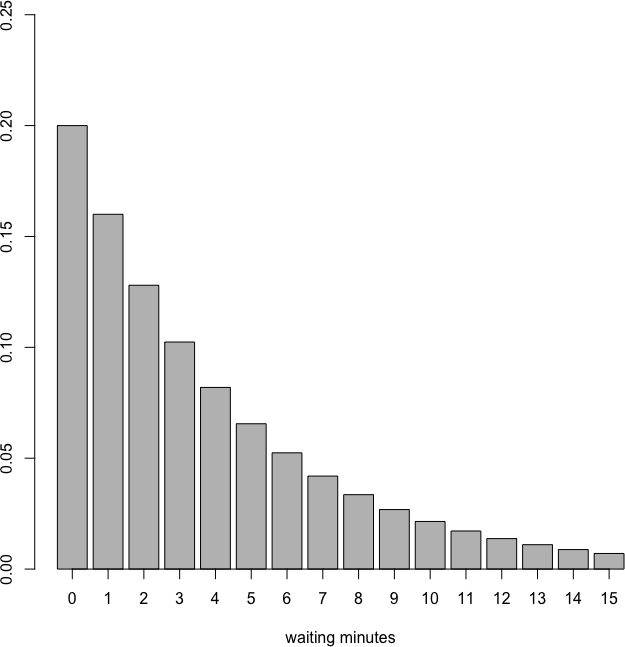
\includegraphics[width=\linewidth]{Images/MaxEnt.png}\end{center}
\end{Exemple}

\subsection*{Exercices} 
\begin{Exercice} \label{ex3.5.1} Dans cet exercice, vous étudierez l'effet possible du choix de la distribution a priori sur les conclusions.
\begin{enumerate}[noitemsep,label=(\alph*)]
	\item Supposons que vous possédez une pièce de monnaie que vous savez qu'elle a été frappée par le gouvernement fédéral et pour laquelle vous n'avez aucune raison de soupçonner de l'altération de toute sorte. Votre croyance a priori sur l'équité de la pièce est donc fort. Vous lancez la pièce 10 fois et
    enregistrez 9 $F$(ace). Quelle est la probabilité que vous prévoyez d'obtenir 1 $F$ au 11ème lancement? Expliquez soigneusement votre réponse; justifiez votre choix de préalable. Comment votre réponse changerait-elle (le cas échéant) si vous utilisez un point de vue fréquentiste?.
	\item Un mystérieux inconnu vous tend une pièce différente, celle-ci faite d'un matériau étrange au toucher, sur laquelle on trouve les mots "l'Association de Global Tricksters" Vous lancez la pièce 10 fois et enregistrez à nouveau 9$F$. Expliquez soigneusement votre réponse; justifier votre choix de la distribution a priori. Remarque: utilisez la distribution a priori de l'exemple \ref{Ex:unusualprior}.
\end{enumerate}
\end{Exercice}